\documentclass[10pt]{article}
\usepackage[polish]{babel}
\usepackage[utf8]{inputenc}
\usepackage[T1]{fontenc}
\usepackage{amsmath}
\usepackage{amsfonts}
\usepackage{amssymb}
\usepackage[version=4]{mhchem}
\usepackage{stmaryrd}
\usepackage{graphicx}
\usepackage[export]{adjustbox}
\graphicspath{ {./images/} }

\title{XIX Konkurs Matematyczny St@ś \\
 XIV LO im. Stanisława Staszica }

\author{}
\date{}


\begin{document}
\maketitle
3 czerwca 2019 roku

Na rozwiazanie poniższych zadań masz 90 minut. Kolejność rozwiazywania tych zadań jest dowolna.\\
Wszystkie zadania sa jednakowo punktowane. Maksymalna liczbę punktów mȯ̇e uzyskać jedynie petne rozwiazanie, z uzasadnieniem \(\boldsymbol{i}\) odpowiedziq.\\
Używanie korektora i korzystanie z kalkulatora jest niedozwolone.

\begin{enumerate}
  \item Różnica między \(\frac{5}{12}\) pierwszej liczby i \(\frac{5}{12}\) drugiej liczby jest równa \(\frac{3}{8}\). Ile jest równa różnica między \(\frac{4}{7}\) tej pierwszej liczby i \(\frac{4}{7}\) drugiej liczby?
  \item Akwarium w kształcie prostopadłościanu całkowicie wypełnione wodą waży 108 kg . To samo akwarium napełnione wodą do połowy waży 57 kg . Ile waży puste akwarium?
  \item Jednakowym literom należy przyporządkować jednakowe cyfry, różnym różne. Wyznacz \(A, C, E, P, R, S, U\), aby działanie było poprawne.
\end{enumerate}

\[
\begin{array}{r}
U S S R \\
+U S A \\
\hline P E A C E
\end{array}
\]

\begin{enumerate}
  \setcounter{enumi}{3}
  \item Dany jest trójkąt równoramienny \(A B C(A B=B C)\). Punkt \(E\) leży na boku \(B C\). Punkty \(D, F\) leżą na boku \(A B\) (punkt \(D\) leży bliż̇ej wierzchołka \(B\), a punkt \(F\) bliżej wierzchołka \(A\) ). Zachodzą równości odcinków
\end{enumerate}

\[
B D=D E=E F=F C=A C .
\]

Obliczyć kąty trójkąta \(A B C\).\\
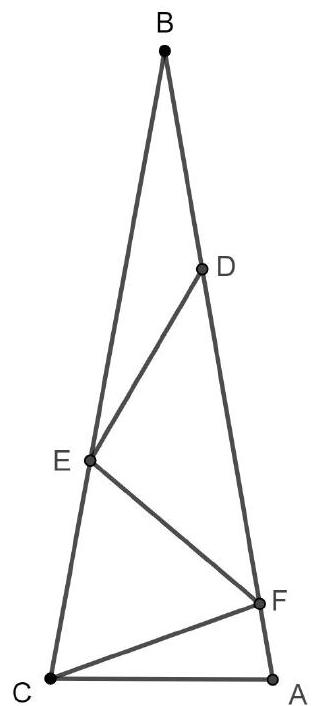
\includegraphics[max width=\textwidth, center]{2024_11_21_74036bdc35e96c893761g-1}\\
5. Wyznaczyć dwie ostatnie cyfry liczby sześciocyfrowej \(5236 x y\) wiedząc, że jest ona podzielna przez 7, 8 i 9.


\end{document}